\chapter{水 肿}

人体血管外组织间隙过多体液积聚时,则形成水肿,此种液体称为水肿液。不包括内脏器官的水肿,如脑水肿、肺水肿等。

产生水肿的主要因素有:①钠和水的异常潴留;②毛细血管滤过压升高;③毛细血管通透性增加;④血浆胶体渗透压降低;⑤淋巴回流受阻碍;⑥组织压力降低。

临床上全身性水肿的主要病理生理学基础是钠和水的异常潴留。一般认为,首先是钠潴留,其次才是水潴留。引起水和钠潴留的机制,如水、钠潴留中的肾性因素(如肾小球的滤过功能与排钠的关系、肾小管的重吸收功能与排钠的关系),水肿形成的内分泌因素(如醛固酮、抗利尿激素与水、钠潴留的关系等),容量感受器(volume
receptor)、容量自体稳定(volume
homeostasis)与水肿的关系等问题受到注意。

有人认为局限性水肿的发生,取决于该处毛细血管的压力梯度(pressure
gradient),即驱使液体离开血管的压力与重新进入血管的压力之差。

在大多数水肿中,肾性水钠异常潴留是水肿发生的主要原因,而毛细血管的压力梯度仅决定水肿的定位。

依照水肿的性质可区分为下列几种:

\section{(一)压陷性水肿与非压陷性水肿}

压陷性水肿是由于体液渗聚于皮下疏松结缔组织间隙所致;非压陷性水肿是由于慢性淋巴回流受阻(如丝虫病象皮肿)、黏液性水肿等所致。

\section{(二)炎症与非炎症水肿}

炎症与非炎症水肿临床一般不难鉴别,炎症水肿以局部潮红、灼热、疼痛与压痛为特征,属于局部性水肿。

\section{(三)全身性水肿与局限性水肿}

当身体内各部分(主要是皮下组织)的血管外组织间隙均有体液积聚时,称为全身性水肿。由于水肿液在体内各组织中呈弥漫性分布,即使有一定量的液体潴留,早期仍可无肉眼可见的水肿,但患者体重可增加。因此,如患者有迅速的体重增加,而无任何原因可解释时,可认为是水肿的最早表现。体液积聚于局部组织间隙中时,称为局限性水肿。

临床上能引起全身性或局限性水肿的疾病繁多(表\ref{tab11-1})。现分节讨论于下。

\begin{longtable}{c}
 \caption{水肿疾病的分类}
 \label{tab11-1}
 \endfirsthead
 \caption[]{水肿疾病的分类}
 \endhead
 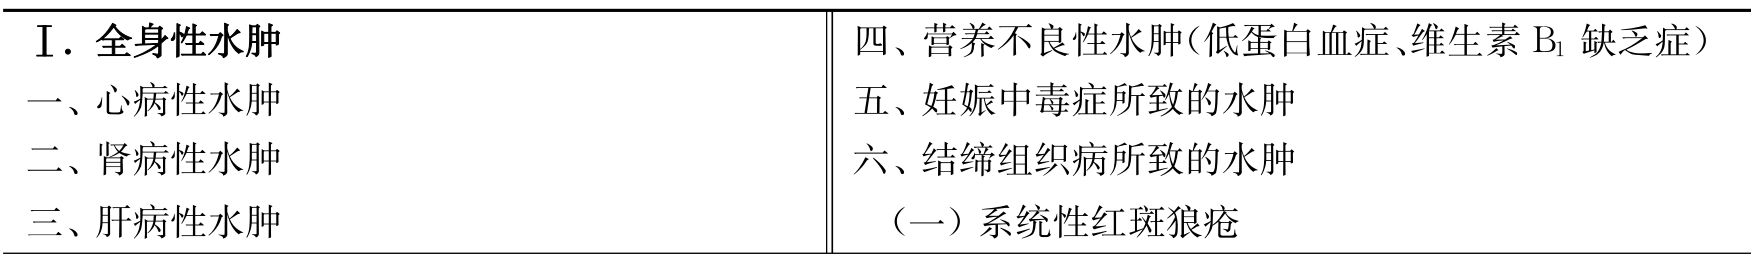
\includegraphics[width=\textwidth,height=\textheight,keepaspectratio]{./images/Image00079.jpg}\\
 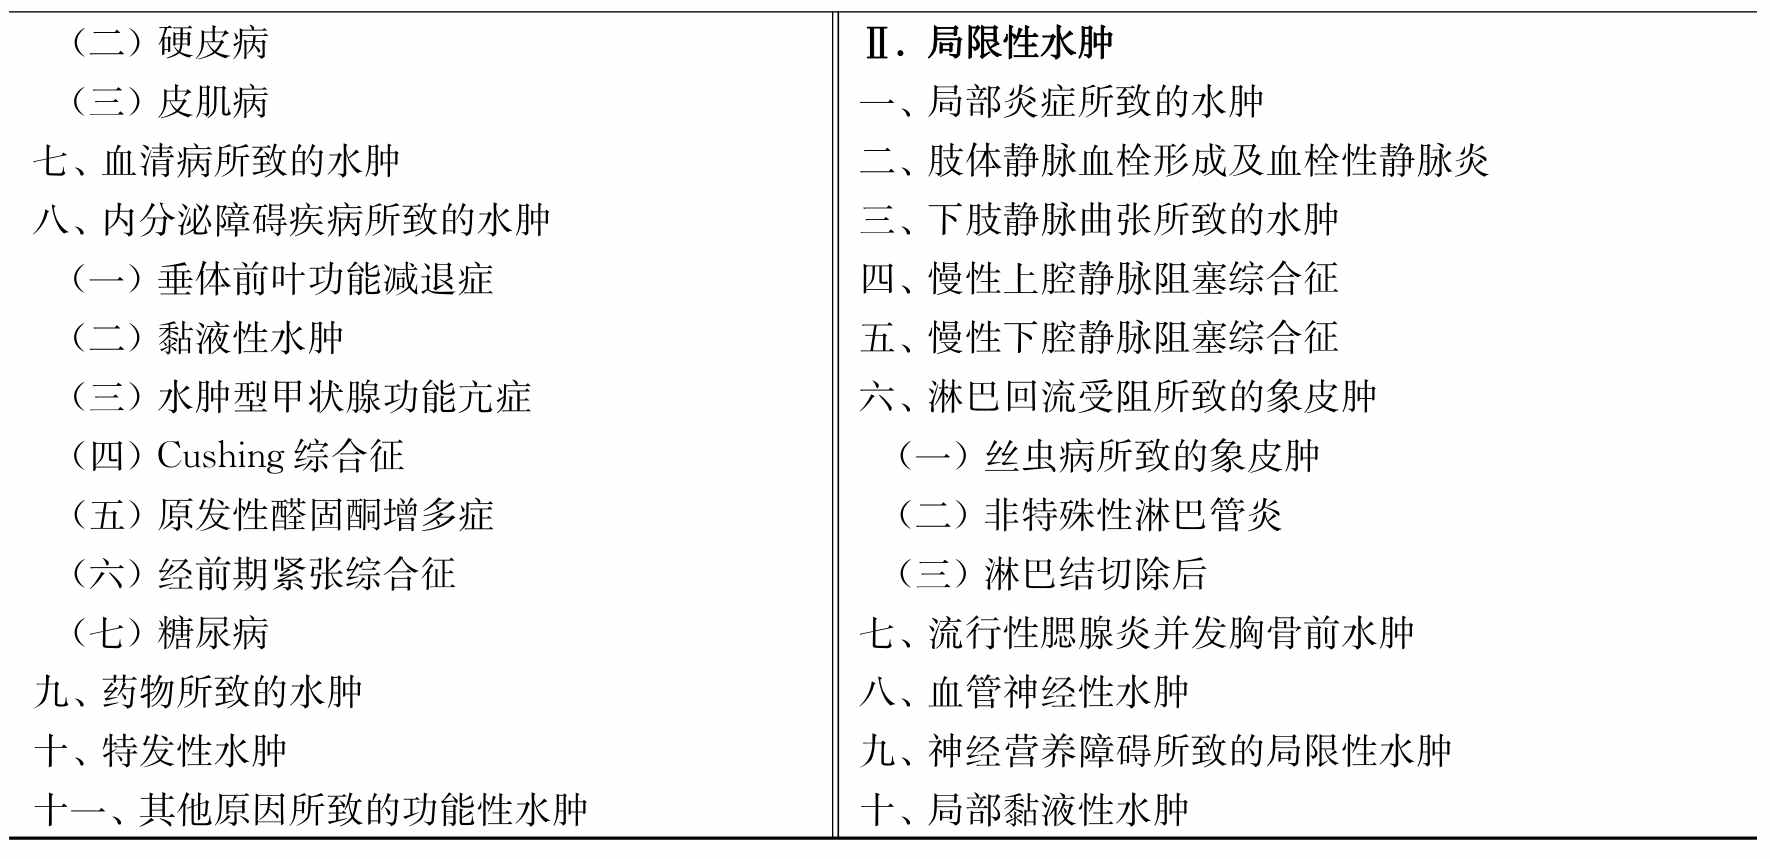
\includegraphics[width=\textwidth,height=\textheight,keepaspectratio]{./images/Image00080.jpg}
 \end{longtable}

\protect\hypertarget{text00104.html}{}{}

\section{37 全身性水肿}

\subsection{一、心病性水肿}

心病性水肿一般认为是右心衰竭的表现。主要是心衰引起有效循环血量减少、肾血流量减少、继发性醛固酮增多引起钠水潴留,以及静脉淤血、毛细血管滤过压增高、组织液回吸收减少所致。前者确定水肿程度,后者决定水肿部位。由于心力衰竭程度不同,心病性水肿可自轻度的踝部水肿以至严重的全身性水肿。水肿的先兆往往表现为体重迅速增加。

心病性水肿的特点是首先发生于下垂部位,为压陷性。非卧床患者的水肿首先出现于下肢,尤以踝部较明显;卧床患者的水肿则首先出现于骶部。严重患者可发生全身性水肿合并胸腔、腹腔及心包积水。如心力衰竭患者出现面部水肿,表明病情严重,且常提示合并营养不良及肝脏受损所致血清白蛋白过低的情况存在。

心病性水肿的诊断主要根据患者的心脏病病史、体征及慢性右心衰竭的临床表现,一般不难确定。

慢性缩窄性心包炎也可引起水肿、淤血性肝大、腹水等体征。若其临床表现不典型,可误诊为肝硬化。慢性缩窄性心包炎有显著的静脉压升高,虽可有肝功能损害,但其程度较轻,肝大而表面平滑。

原发性心肌病在慢性病程中可出现充血性心力衰竭的临床病象,或表现为类似慢性缩窄性心包炎的临床病象,常伴有水肿(主要发生于下肢)。

\subsection{二、肾病性水肿}

肾病性水肿的特点是疾病早期只于早晨起床时发现眼睑或颜面水肿,逐渐发展为全身性水肿。

水肿、血压升高与尿改变(血尿、蛋白尿与管型尿),一般是诊断肾炎性水肿的有力证据。钠水潴留是肾性水肿的基本机制。急性肾炎引起水肿的机制几乎是肾性钠水异常潴留。肾病综合征常以重度全身性水肿、重度蛋白尿、低蛋白血症与血清胆固醇增高等为特征,其水肿的分布与体位关系不大。肾病综合征水肿的机制主要是大量蛋白尿所致的低蛋白血症,以及钠水潴留、肾小管重吸收钠过多等,后者可能由于血容量减少引起继发性醛固酮增多所致。肾病性水肿需与心病性水肿相鉴别,鉴别要点见表\ref{tab11-2}。

\begin{table}[htbp]
\centering
\caption{肾脏性水肿与心病性水肿的鉴别}
\label{tab11-2}
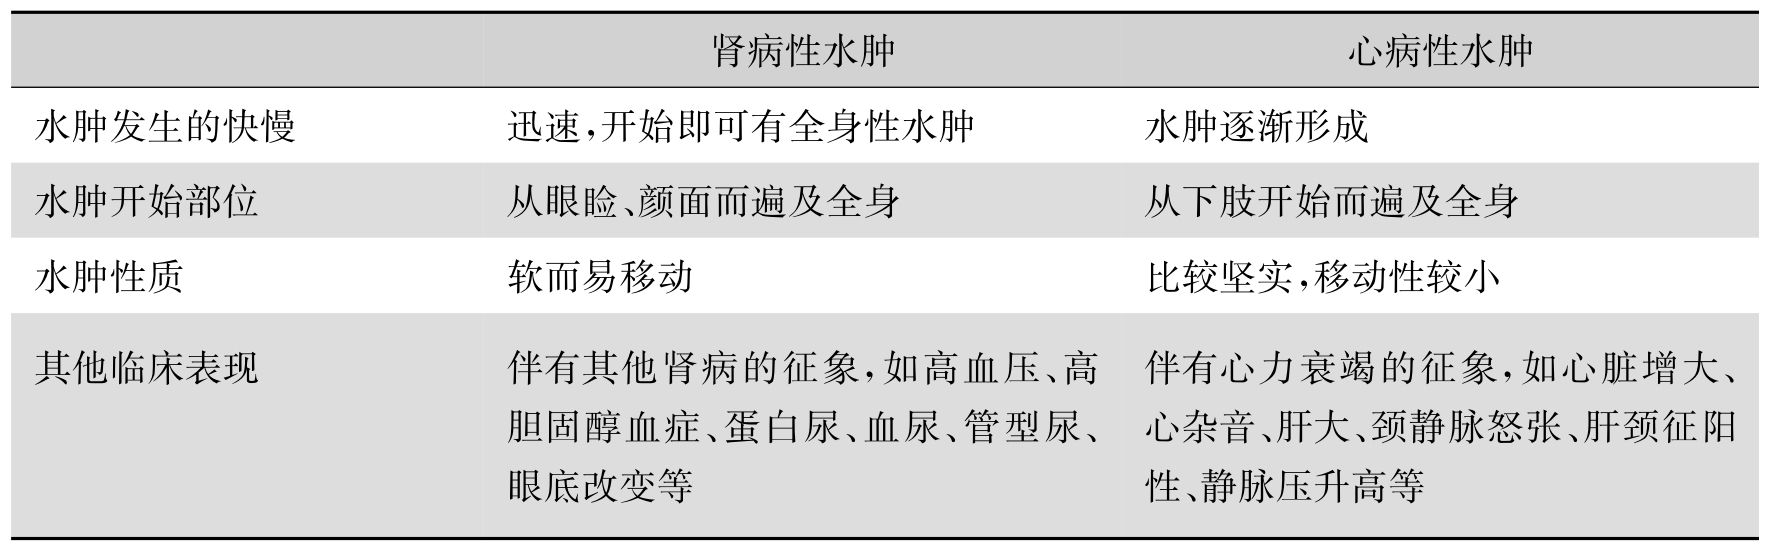
\includegraphics[width=5.91667in,height=1.84375in]{./images/Image00081.jpg}
\end{table}

\subsection{三、肝病性水肿}

肝硬化在腹水出现之前可先有轻度下肢水肿,疾病发展严重时可出现腹水,甚至全身水肿。低蛋白血症、门脉高压症、肝淋巴回流障碍、继发醛固酮增多等因素是水肿和腹水形成的主要机制。肝脏病时出现全身水肿,常提示有营养不良与较重的肝功能损害存在。

\subsection{四、营养不良性水肿}

营养缺乏性水肿主要由于长时间负氮平衡,低蛋白血症引起血管胶体渗透压降低所致。水肿发生前常有消瘦、体重减轻,一般给予高热量高蛋白膳食,水肿不久便消退,据此不难确定诊断,但营养缺乏水肿不少合并维生素B\textsubscript{1}
缺乏症,这也可为水肿的附加原因。

维生素B\textsubscript{1}
缺乏症伴有水肿者称为湿性型脚气病。可累及消化、神经、心血管系统,其主要症状为纳差、手足麻木感、衰弱、四肢运动障碍、膝反射消失与全身性水肿等。重病者可出现心脏症状(脚气病性心脏病),如不积极治疗,可危及生命。维生素B\textsubscript{1}
缺乏症所致的水肿往往首先出现于踝部,病情进展时向上发展。下肢、阴囊、腹壁等处的水肿以及浆膜腔积液并不罕见。患者平卧时下肢水肿减少,但可蔓延及颜面。尿量减少,但无蛋白尿,这可与肾病性水肿鉴别。维生素B\textsubscript{1}
主要来源于食物,询问病史如存在维生素B\textsubscript{1}
摄入减少或丢失消耗过多的情况有助于诊断本病(例如长期吃精白大米与偏食习惯,慢性腹泻以致吸收障碍,发热以及其他慢性消耗疾病以致需要增多等)。应用维生素B\textsubscript{1}
治疗后,而病情迅速改善者,对诊断有一定帮助。

维生素B\textsubscript{1}
缺乏可引起周围小动脉扩张,心搏出量增多,静脉压升高,这时不论有无心肌功能损害都可以出现水肿。

\subsection{五、妊娠中毒症所致的水肿}

妊娠中毒症可发生于妊娠20周后,多发生于妊娠24周以后,初产妇常见。水肿程度可自轻度至全身性水肿。水肿、蛋白尿、血压升高与眼底改变是此症的主要表现,严重时可出现抽搐与昏迷。水钠潴留和毛细血管渗透性增加等因素,被认为是水肿的重要原因。

正常妊娠中期以后,孕妇也常有不同程度的下肢水肿,这主要由于增大的子宫压迫盆腔静脉,引起下肢静脉回流障碍所致,但无蛋白尿与血压升高,这可与妊娠中毒症相区别。

\subsection{六、结缔组织病所致的水肿}

\subsubsection{(一)系统性红斑狼疮}

系统性红斑狼疮是侵犯皮肤和多脏器的一种全身性自身免疫性疾病,发病可急可缓,早期轻症的患者往往仅有单一系统或器官受累的不典型表现,随着病程的发展可表现为多个系统和器官受累的临床症状。可能出现轻度水肿,以面部及踝部较多见,也可为全身性。水肿形成与全身性血管病变及血清白蛋白降低有关。当合并狼疮性肾炎时亦可出现类似肾病性水肿的表现。

\subsubsection{(二)硬皮病}

硬皮病是少见的疾病,起病常缓慢。可分弥漫型、局限型及肢端硬化型三型。弥漫型的早期,患者感觉全身不适、关节痛、神经痛、微热以及皮肤病变,首发症状多为肢端动脉痉挛现象(雷诺现象)。病程中逐渐出现肺、消化道、肾脏及心脏等脏器损害。

此病典型的皮肤病变经过三个时期:水肿期、发硬期及萎缩期。

\paragraph{1.水肿期}

皮肤肥厚及紧张,光滑发亮,先由手部及足部开始,手指常呈“腊肠样”,伴晨僵,可有关节痛,并可出现腕管综合征。病变发展逐渐累及颈、面及躯干。此种弥漫性水肿属于非压陷性水肿,表现为两侧皮肤呈淡黄色或黄白色的对称性肿胀而失去皱纹。患者呈一种黄白色而有蜡样光泽的水肿面容。

\paragraph{2.发硬期}

病程经过中皮肤因纤维性变而变硬,紧张度增加,不易被捻起,手指屈伸不自如,面部皮肤板硬而缺乏表情。皮色黄褐,有时发生灰褐色色素沉着。

\paragraph{3.萎缩期}

经年累月之后,皮肤色素沉着及发硬程度逐渐加重,全身皮肤、皮下组织与肌肉均萎缩,毛发脱落,汗闭,易继发顽固性溃疡。面颈部皮肤受累时,可形成“面具脸。”

皮肤活体组织检查对此病的诊断有重要帮助。

\subsubsection{(三)皮肌炎}

皮肌炎,尤其是急性皮肌炎常出现轻度水肿(参见第2.2节)。

\subsection{七、血清病所致的水肿}

血清病是由于注射动物血清而引起的Ⅲ型变态反应性疾病。患者注射动物血清(最常为马血清)经一定的潜伏期后(多为1~3周),出现发热、皮疹、关节痛、淋巴结肿痛等症状。有些患者出现眼睑、面部、手足等处的水肿,体重增加,极少数患者可出现喉头水肿。肾功能一般正常。尿液检查可有短暂的蛋白尿与少数管型。

\subsection{八、内分泌代谢障碍疾病所致的水肿}

\subsubsection{(一)垂体前叶功能减退症}

垂体前叶功能减退症大多由产后大出血引起。当促甲状腺激素减少或缺乏时,患者可出现典型黏液性水肿的面容,呈皮肤水肿、增厚、干而有鳞屑,毛发脱落、稀疏。

\subsubsection{(二)黏液性水肿}

甲状腺功能减退症(简称甲减)发生时,黏多糖在组织和皮肤堆积,表现为黏液性水肿,可见于儿童或成年人。幼年型黏液性水肿多为原发性。成人型黏液性水肿多为继发性,可见于:①甲状腺功能亢进症治疗后(手术、放射性核素131碘治疗、长期服过量抗甲状腺药物);②继发于垂体前叶功能减退症或(及)下视丘损伤;③与慢性甲状腺炎或甲状腺自身免疫疾病有关。原因未明的所谓特发性甲减并不少见,常易漏诊。临床上特别是年轻人原因未明的水肿,须注意本病的可能性,以免漏诊。

黏液性水肿的特点是皮肤呈非压陷性水肿,水肿处皮肤苍白或蜡黄,轻者颜面及下肢出现水肿,严重病例全身皮下组织均可累及,甚至可出现心包积液、胸腔与腹腔积液。患者可有特征性的面部表现:表情淡漠呆板、睑面水肿,鼻宽,唇厚,舌大,言语缓慢,发音不清。临床上如患者有未能解释的全身乏力、怕冷、皮肤苍黄而干燥、水肿、毛发脱落、反应迟钝、便秘、女性月经紊乱与中等度贫血等情况时,应考虑本病。

实验室检查发现TSH增高,TT\textsubscript{4} 、FT\textsubscript{4}
减低,原发性甲减诊断可成立;如TSH正常,FT\textsubscript{4}
减低,考虑为垂体性甲减或下丘脑性甲减,需做TRH试验来区分。

黏液性水肿须与假性黏液性水肿鉴别。后者可发生于患有持久性高血压的患者,是发生于面部、手部或足部的轻度水肿,面色苍白,常兼有肥胖症,而并无心、肾、肝各脏器功能不全的病征。假性黏液性水肿用甲状腺素治疗无效。

\subsubsection{(三)水肿型甲状腺功能亢进症}

本型甲状腺功能亢进症罕见,患者有甲亢的表现,并伴有水肿。水肿常自下肢胫前开始,向上蔓延,为非压陷性,利尿药治疗疗效不佳。但在甲亢病情控制之后,水肿亦随之消退。

\subsubsection{(四)Cushing综合征}

因肾上腺皮质分泌过多皮质素,引起水钠潴留,少数病例出现面部及下肢轻度水肿,水肿可为早期症状,易误诊为慢性肾炎,但患者通常有向心性肥胖、肌肉消耗、皮肤紫纹、骨质疏松、糖耐量低下等。

\subsubsection{(五)原发性醛固酮增多症}

原发性醛固酮增多症时,由于肾上腺皮质分泌醛固酮及去氧皮质酮过多,肾小管钠水重吸收增加,出现高血压、低血钾、高血钠、血浆容量增加、多尿等症状,少数病例可出现下肢及面部轻度水肿。但非本病的主要症状。

\subsubsection{(六)经前期紧张综合征}

本综合征的临床表现颇为复杂,水肿是常见的症状,但神经症症状最常见而突出------患者兴奋性增高、烦躁、易怒、常失眠,常有弥漫性头痛,有时偏头痛,易疲乏、懒散、思想不集中。体重可增加1~2kg或更多,伴眼睑、踝部与手部轻度水肿。可有乳房胀痛与盆腔部沉重感,偶尔出现胆道运动功能障碍。上述症状多于月经开始前7~14天出现,而于月经来潮时消退,但少数也可于月经周期或其他期间出现。月经来潮之后,患者排尿量增加,水肿和其他症状逐渐消退。

\subsubsection{(八)糖尿病}

水肿发生原因是多方面的,如糖尿病性肾病、周围神经炎、营养不良、肥胖、药物等原因。

\subsection{九、药物所致的水肿}

由于应用药物而引起的水肿临床上并不少见,其特点是水肿在用药后发生,停药后不久消失。例如应用肾上腺皮质激素、甘草、雄激素、雌激素、胰岛素、硫脲、过氯酸钾、萝芙木等药物时,均可引起钠水潴留而导致水肿。

\subsection{十、特发性水肿}

如水肿发生而无任何明显的、已知的原因,称为特发性水肿。特发性水肿目前已作为一种有些特殊的、原因未明或原因尚未确定的(可能有一种以上原因)综合征。此综合征几乎只发生于妇女,水肿往往有和月经有关的周期性,其主要发病机制曾被考虑为内分泌功能失调以及对直立体位的反应异常。患者在直立位时血浆中肾素活性增高,显著超过正常人,提示继发性醛固酮增多症。继发性醛固酮增多症似是肾小管重吸收增加与肾性水钠潴留的重要原因,但水肿的真正原因迄今尚未明了。

特发性水肿患者的体位适应性,与健康女性比较有明显的差别。患者晨间与晚间的体重差别较大,晨起体重较晚间明显减轻。患者取直立位时收缩压下降较多,下肢体积增加较多,血浆肾素活性较高,尿中醛固酮排量较多。多数患者无排卵周期,并有孕酮不足与雌激素相对增多。多数有月经前水肿。直立位的血流动力学与内分泌反应促进了病情,并引起过度的钠潴留,这种反应可促发已存在着的潜在性因素而发生水肿。

诊断特发性水肿须仔细除外其他病因,如心、肾、肝等脏器疾病以及营养不良所导致的水肿。采取卧床休息,弹性长袜,限制食盐,应用拟交感神经药、盐类利尿剂、醛固酮抑制剂、孕酮等,可使水肿消退。

立卧位水试验*可有助于特发性水肿的诊断。特发性水肿时此试验常呈现阳性。

特发性水肿兼有单纯性肥胖症,则为水潴留性肥胖症。

*立卧位水试验
嘱患者清晨空腹排尿后,于20分钟内饮水1000ml,然后每小时排尿一次,连续4次,测定总尿量。第一天取卧位(不用枕头),第二天取直立位(即活动或工作)以同样方法测定尿量,立位时尿量低于卧位尿量50\%以上为阳性。

\subsection{十一、其他原因所致的功能性水肿}

有些人在高温环境下有发生轻度水肿的倾向,并可于夏季出现,反复多年。这可能由于温热刺激引起的体表血管扩张,动脉血流量增加和浅静脉的扩张、淤滞,致毛细血管滤过压增高,体液在皮下疏松结缔组织间隙渗聚而形成轻度水肿。水肿通常发生于足、手等处。

肥胖者的水肿倾向往往大于消瘦者。其原因主要有:①脂肪是良好的隔热体,肥胖者散热比较困难,因而往往须借助于周围血管的扩张;②肥胖者不喜活动,也促使下肢静脉压升高,致毛细血管滤过压升高;③皮下脂肪组织增多,可减弱对浅静脉的支撑作用,而易于扩张、淤滞。

“旅行者水肿”可见于久坐或长时间站立行走的旅行者。其原因过去认为坐或站立时间较长,由于重力的关系,下肢(及下垂的上肢)静脉回流受影响,致增加了毛细血管的滤过压,体液在皮下组织间隙渗聚所致。近年发现直立位时醛固酮分泌增加,对水肿形成有关。

“老年性水肿”是由于老年人体质及器官功能随年龄的增长而逐渐衰减,机体代谢逐渐减低,维持内环境稳定的能力下降。因此即使在心、肝、肾、肺及内分泌功能尚未达到衰竭的状态时,在某些因素的影响下,如环境、体位、水钠过度负荷等,都可能促进水肿的发生。

间脑综合征可出现轻度水肿,多累及下肢。水肿也可为一侧性,提示和自主神经功能紊乱有关。

\protect\hypertarget{text00105.html}{}{}

\section{38 局限性水肿}

\subsection{一、局部炎症所致的水肿}

由于疖、痈、丹毒、蜂窝织炎等局部炎症所致的水肿,常伴有局部红、热及压痛,诊断不难。

\subsection{二、肢体静脉血栓形成及血栓性静脉炎}

肢体静脉血栓形成是静脉内有血栓形成;血栓性静脉炎是静脉发炎伴有血栓形成。两者均可出现局限性水肿。肢体浅组织静脉血栓形成和血栓性静脉炎的重要区别是:后者除有局限性水肿外,还有局部炎症表现。深部组织静脉血栓形成或血栓性静脉炎时,因两者局部均有疼痛、压痛与水肿等表现,故较难区别,但前者多无发热而后者常有发热。

\subsection{三、下肢静脉曲张所致的水肿}

下肢静脉曲张多发生在小腿,静脉呈高度扩张、弯曲、隆起,尤以站立时更明显,患肢踝部及足背往往出现水肿,其发生与静脉回流不畅、局部血管流体静压增高有关。晚期局部皮肤可有萎缩、色素沉着及慢性溃疡形成。

\subsection{四、慢性上腔静脉阻塞综合征}

本综合征国内报告大多由恶性肿瘤(肺癌、恶性淋巴瘤)引起;少数为“良性”阻塞,由慢性结核性纵隔炎、原发性上腔静脉血栓形成和白塞病等引起。鉴别其为恶性或“良性”,对治疗与预后有重要意义。

水肿出现于面、颈、上肢及上胸部,形成所谓“披肩状”水肿。患者颈静脉怒张,前胸部表浅静脉扩张、血流方向向下,也常有肝大,或兼有发绀、气促、咳嗽与声音嘶哑。上肢静脉压显著升高。严重病例可有全身性水肿、胸水、腹水。上腔静脉造影可显示阻塞的部位。

本综合征如由慢性纵隔炎或血栓性静脉炎引起,患者有上肢静脉压高、水肿、肝大等表现,而心脏正常、X线检查又无纵隔增宽的征象,易与慢性缩窄性心包炎混淆,选择性上腔静脉造影术有助于鉴别诊断。

\subsection{五、慢性下腔静脉阻塞综合征}

引起下腔静脉阻塞的原因有血栓形成、恶性肿瘤压迫或肿瘤组织侵入静脉内引起阻塞等。本综合征有腹胀、腹壁静脉曲张、下肢与阴囊水肿,伴有肝或脾大,临床上易被误诊为肝硬化,但有下列不同点可资鉴别:①本综合征腹壁静脉曲张的血流均向上,而肝硬化时脐以上水平者血流向上,而脐以下水平者血流向下;②本综合征时下肢水肿出现较早或与下肢静脉曲张同时出现,同时下肢静脉压升高;③本综合征时有精索静脉曲张;④本综合征时肘静脉血氨与腹壁静脉血氨数值相近,而肝硬化时腹壁静脉血氨可较肘静脉者为高;⑤必要时作下腔静脉造影,本综合征显示阻塞现象。

\subsection{六、淋巴回流受阻所致的水肿}

淋巴回流受阻可引起该处淋巴系统回纳区域的局限性水肿。其中以丝虫病所致的慢性淋巴管炎最常见,以后并可演变成象皮肿。

\subsubsection{(一)丝虫病所致的象皮肿}

丝虫寄生于淋巴系统引起淋巴管炎及淋巴结炎,由于影响淋巴液回流以致出现局部性水肿。如淋巴血流长期受阻合并反复继发性感染时,便可逐渐形成象皮肿。

象皮肿是晚期丝虫病特征性表现之一,患部皮肤粗糙与增厚,如皮革样,并起皱褶,皮下组织也显著增厚。象皮肿以下肢最常见,次为阴囊、阴唇、上肢等部。马来丝虫主要寄生于浅部淋巴系统,故以四肢淋巴管炎与象皮肿较为常见。班氏丝虫不仅寄生于四肢淋巴系统,同时还寄生于泌尿生殖系的淋巴系统,故除下肢与阴囊出现淋巴管炎、象皮肿外,还可有乳糜尿或乳糜血尿。诊断须根据患者的临床表现、血中检出微丝蚴以及患部皮肤活组织检查所见等。

\subsubsection{(二)非特异性淋巴管炎}

非特异性淋巴管炎及其后所引起的局部性水肿,临床上少见,且诊断大多困难。

\subsubsection{(三)淋巴结切除后}

在癌性、结核性等淋巴结肿大切除术后,有时也可引起淋巴回流受阻,而出现类似象皮肿的局部性水肿。例如乳腺癌根治术后,可发生同侧上肢水肿甚至象皮肿样改变。淋巴造影有助于诊断。

\subsection{七、流行性腮腺炎并发胸骨前水肿}

流行性腮腺炎并发胸骨前水肿临床上少见。水肿多为凹陷性,其范围大小不等,有时直径可达7.5cm,水肿常在病期第5~6天发生,平均持续约5天而消退。水肿的皮肤大致正常,有时可呈暗红色,可有明显压痛或无压痛。其产生原因可能与胸骨上区的淋巴回流受阻有关。本病多见于流行性腮腺炎流行期间的严重患者。

\subsection{八、血管神经性水肿}

血管神经性水肿属于变态反应性疾病,患者往往有对药物、食物或周围环境过敏的历史,发病前少有前驱症状。该病水肿的特点是突然发生的、无痛的、硬而富有弹性的局限性水肿。水肿的皮肤呈苍白色或蜡样光泽,水肿的中央部微凹下,边缘无明显的界限。

遗传性血管性水肿(HAE)是一种常染色体显性遗传病,但文献报告约20\%患者无家族病史。遗传性血管性水肿可发生于任何年龄,但多见于成年早期。常在外伤或受撞击后10余小时发生皮肤水肿,多见于面部及四肢,持续1~3天可自行消退,但可反复发作,如累及咽喉部可发生喉头水肿引起猝死。血清酯酶抑制蛋白、C4抗原、C2抗原测定值降低提示本病的可能性。C4抗原量减少是诊断普通型HAE的重要依据。

血管神经性水肿分两型:

\subsubsection{1.普通型}

此型水肿的常见症状是颜面、口唇和舌等部位的皮肤或黏膜呈急性暂时性局限性水肿;如水肿侵及喉头声门时,可引起致命的声门水肿。

\subsubsection{2.神经精神型}

此型较单纯型少见。其常见的症状是患者突然发生的倦怠、头痛、发作性嗜睡、头晕、暂时性眼肌瘫痪与视力减退等症状。

本病的诊断主要根据:①发病突然,无任何前驱症状,部分患者过去有同样发作的病史;②水肿的性质如上述,局部淋巴结不肿大,体温无改变,白细胞总数一般不增多,但嗜酸性粒细胞可稍增多;③除外外伤、感染及昆虫咬伤等所致的局限性水肿。

\subsection{九、神经营养障碍所致的局限性水肿}

某些中枢神经系统疾病(如脑出血后),其瘫痪或麻木的患肢可发生轻度乃至中度的水肿,此可能由于神经营养障碍引起局部毛细血管渗透性增加所致。

\subsection{十、局部黏液性水肿}

局部黏液性水肿是较少见的内分泌疾病,大概占甲状腺功能亢进症的4\%。国内已有多例报告。多发生于突眼性甲状腺肿中年纪较大的男性。以甲状腺手术后或复发病例较多见,也可见于甲状腺功能正常或减退者。局部黏液性水肿多发生在下肢,尤多见于胫骨前与足背的皮肤,此外,眼睑、阴囊、前额、肩部或背部也可出现。皮肤结节状增厚隆起,质硬,呈红、棕、紫或正常颜色,粗糙,毛孔粗大如猪皮样,局部温度较低,不痛,多对称发生。病因可能与垂体分泌促甲状腺素过多,引起局部透明质酸分泌较多有关;局部注射透明质酸酶可使患处结节减退并皮肤凹陷。近年来也有人提出,可能与体内产生的自身免疫抗体------长效甲状腺刺激素(longacting
thyroid stimulator,LATS)有关。

此病须与下肢象皮肿区别,一般结合病史及体征不难鉴别,皮肤活体组织检查也有助于确诊。

\protect\hypertarget{text00106.html}{}{}

\section{参考文献}

1.Bahloul M,Chaari AN,Kallel H,et al.Neurogenic pulmonary edema due
to traumatic brain injury:evidence of cardiac dysfunction.Am J Crit
Care,2006;15(5):462-70.

2.Bhagat N,Grigorian RA,Tutela A,et al.Diabetic
macularedema:pathogenesis and treatment.Surv
Ophthalmol,2009;54(1):1-32.

3.Bork K.Angioedema.Immunol Allergy Clin North Am,2014;34(1):23-31.

\protect\hypertarget{text00107.html}{}{}

